%% fig_vgcounts.tex   (generated by make_round41.py; do not edit by hand)
%% Hodge classes of degree r on the very general member against h^{r/2,r/2} (thm:vgvandermonde(iii)).
\documentclass[tikz,border=8pt]{standalone}
\usepackage{amsmath,amssymb}
\usetikzlibrary{arrows.meta,calc,decorations.pathreplacing}
%% palette.tex -- shared colour definitions for the figures
\definecolor{PInk}{RGB}{26,32,44}
\definecolor{PBlue}{RGB}{37,82,139}
\definecolor{PTeal}{RGB}{23,127,125}
\definecolor{POchre}{RGB}{193,138,44}
\definecolor{PClay}{RGB}{178,74,58}
\definecolor{PSlate}{RGB}{108,122,137}
\definecolor{PViolet}{RGB}{110,86,150}
\definecolor{WBlue}{RGB}{223,234,246}
\definecolor{WTeal}{RGB}{220,238,236}
\definecolor{WOchre}{RGB}{250,240,218}
\definecolor{WClay}{RGB}{247,229,224}
\definecolor{WSlate}{RGB}{238,241,244}
\definecolor{PMag}{RGB}{158,58,110}
\definecolor{PGrass}{RGB}{62,124,66}
\definecolor{PAmber}{RGB}{214,112,38}
\definecolor{PIndigo}{RGB}{58,64,140}
\definecolor{PRule}{RGB}{176,186,197}

%% shared macros so the standalone figures match the paper
\providecommand{\QQ}{\mathbb{Q}}
\providecommand{\ZZ}{\mathbb{Z}}
\providecommand{\RR}{\mathbb{R}}
\providecommand{\CC}{\mathbb{C}}
\providecommand{\PP}{\mathbb{P}}
\providecommand{\Kx}{K^{\times}}
\providecommand{\HW}{W}
\providecommand{\Nm}{\mathrm{N}}
\providecommand{\Hdg}{\mathrm{Hdg}}
\providecommand{\NS}{\mathrm{NS}}
\providecommand{\cA}{\mathcal{A}}
\providecommand{\cD}{\mathcal{D}}
\providecommand{\cF}{\mathcal{F}}
\providecommand{\cP}{\mathcal{P}}
\providecommand{\cO}{\mathcal{O}}
\providecommand{\cQ}{\mathcal{Q}}
\providecommand{\bbar}[1]{\overline{#1}}
\providecommand{\ch}{\operatorname{ch}}
\providecommand{\End}{\mathrm{End}}
\providecommand{\Ext}{\operatorname{Ext}}
\providecommand{\Supp}{\operatorname{Supp}}

\begin{document}
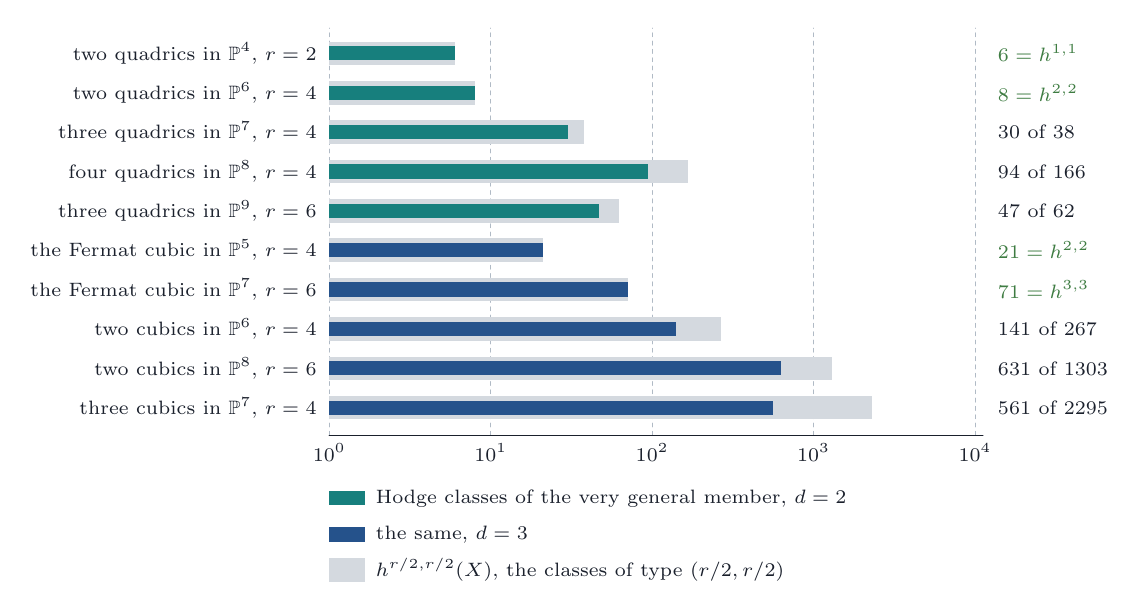
\begin{tikzpicture}[x=1cm,y=1cm,line join=round,line cap=round,
  font=\small,text=PInk,lbl/.style={inner sep=1pt}]
  \draw[PRule,line width=0.35pt,dash pattern=on 1.4pt off 1.6pt] (5.4000,-0.3500) -- (5.4000,4.8200);
  \draw[PRule,line width=0.35pt,dash pattern=on 1.4pt off 1.6pt] (7.4500,-0.3500) -- (7.4500,4.8200);
  \draw[PRule,line width=0.35pt,dash pattern=on 1.4pt off 1.6pt] (9.5000,-0.3500) -- (9.5000,4.8200);
  \draw[PRule,line width=0.35pt,dash pattern=on 1.4pt off 1.6pt] (11.5500,-0.3500) -- (11.5500,4.8200);
  \draw[PRule,line width=0.35pt,dash pattern=on 1.4pt off 1.6pt] (13.6000,-0.3500) -- (13.6000,4.8200);
  \draw[PInk,line width=0.5pt] (5.4000,-0.3500) -- (13.7000,-0.3500);
  \path[fill=PRule!55!white,draw=none] (5.4000,4.3500) rectangle (6.9952,4.6500);
  \path[fill=PTeal,draw=none] (5.4000,4.4100) rectangle (6.9952,4.5900);
  \path[fill=PRule!55!white,draw=none] (5.4000,3.8500) rectangle (7.2513,4.1500);
  \path[fill=PTeal,draw=none] (5.4000,3.9100) rectangle (7.2513,4.0900);
  \path[fill=PRule!55!white,draw=none] (5.4000,3.3500) rectangle (8.6386,3.6500);
  \path[fill=PTeal,draw=none] (5.4000,3.4100) rectangle (8.4281,3.5900);
  \path[fill=PRule!55!white,draw=none] (5.4000,2.8500) rectangle (9.9512,3.1500);
  \path[fill=PTeal,draw=none] (5.4000,2.9100) rectangle (9.4449,3.0900);
  \path[fill=PRule!55!white,draw=none] (5.4000,2.3500) rectangle (9.0744,2.6500);
  \path[fill=PTeal,draw=none] (5.4000,2.4100) rectangle (8.8278,2.5900);
  \path[fill=PRule!55!white,draw=none] (5.4000,1.8500) rectangle (8.1105,2.1500);
  \path[fill=PBlue,draw=none] (5.4000,1.9100) rectangle (8.1105,2.0900);
  \path[fill=PRule!55!white,draw=none] (5.4000,1.3500) rectangle (9.1951,1.6500);
  \path[fill=PBlue,draw=none] (5.4000,1.4100) rectangle (9.1951,1.5900);
  \path[fill=PRule!55!white,draw=none] (5.4000,0.8500) rectangle (10.3743,1.1500);
  \path[fill=PBlue,draw=none] (5.4000,0.9100) rectangle (9.8059,1.0900);
  \path[fill=PRule!55!white,draw=none] (5.4000,0.3500) rectangle (11.7856,0.6500);
  \path[fill=PBlue,draw=none] (5.4000,0.4100) rectangle (11.1401,0.5900);
  \path[fill=PRule!55!white,draw=none] (5.4000,-0.1500) rectangle (12.2896,0.1500);
  \path[fill=PBlue,draw=none] (5.4000,-0.0900) rectangle (11.0354,0.0900);
  \path[fill=PTeal,draw=none] (5.4000,-1.2400) rectangle (5.8500,-1.0600);
  \path[fill=PBlue,draw=none] (5.4000,-1.7000) rectangle (5.8500,-1.5200);
  \path[fill=PRule!55!white,draw=none] (5.4000,-2.2100) rectangle (5.8500,-1.9100);
  \node[lbl,anchor=north,text=PInk,font=\scriptsize] at (5.4000,-0.4200) {$10^{0}$};
  \node[lbl,anchor=north,text=PInk,font=\scriptsize] at (7.4500,-0.4200) {$10^{1}$};
  \node[lbl,anchor=north,text=PInk,font=\scriptsize] at (9.5000,-0.4200) {$10^{2}$};
  \node[lbl,anchor=north,text=PInk,font=\scriptsize] at (11.5500,-0.4200) {$10^{3}$};
  \node[lbl,anchor=north,text=PInk,font=\scriptsize] at (13.6000,-0.4200) {$10^{4}$};
  \node[lbl,anchor=east,text=PInk,font=\scriptsize] at (5.2800,4.5000) {two quadrics in $\PP^{4}$, $r=2$};
  \node[lbl,anchor=west,text=PGrass,font=\scriptsize] at (13.8500,4.5000) {$6=h^{1,1}$};
  \node[lbl,anchor=east,text=PInk,font=\scriptsize] at (5.2800,4.0000) {two quadrics in $\PP^{6}$, $r=4$};
  \node[lbl,anchor=west,text=PGrass,font=\scriptsize] at (13.8500,4.0000) {$8=h^{2,2}$};
  \node[lbl,anchor=east,text=PInk,font=\scriptsize] at (5.2800,3.5000) {three quadrics in $\PP^{7}$, $r=4$};
  \node[lbl,anchor=west,text=PInk,font=\scriptsize] at (13.8500,3.5000) {$30$ of $38$};
  \node[lbl,anchor=east,text=PInk,font=\scriptsize] at (5.2800,3.0000) {four quadrics in $\PP^{8}$, $r=4$};
  \node[lbl,anchor=west,text=PInk,font=\scriptsize] at (13.8500,3.0000) {$94$ of $166$};
  \node[lbl,anchor=east,text=PInk,font=\scriptsize] at (5.2800,2.5000) {three quadrics in $\PP^{9}$, $r=6$};
  \node[lbl,anchor=west,text=PInk,font=\scriptsize] at (13.8500,2.5000) {$47$ of $62$};
  \node[lbl,anchor=east,text=PInk,font=\scriptsize] at (5.2800,2.0000) {the Fermat cubic in $\PP^{5}$, $r=4$};
  \node[lbl,anchor=west,text=PGrass,font=\scriptsize] at (13.8500,2.0000) {$21=h^{2,2}$};
  \node[lbl,anchor=east,text=PInk,font=\scriptsize] at (5.2800,1.5000) {the Fermat cubic in $\PP^{7}$, $r=6$};
  \node[lbl,anchor=west,text=PGrass,font=\scriptsize] at (13.8500,1.5000) {$71=h^{3,3}$};
  \node[lbl,anchor=east,text=PInk,font=\scriptsize] at (5.2800,1.0000) {two cubics in $\PP^{6}$, $r=4$};
  \node[lbl,anchor=west,text=PInk,font=\scriptsize] at (13.8500,1.0000) {$141$ of $267$};
  \node[lbl,anchor=east,text=PInk,font=\scriptsize] at (5.2800,0.5000) {two cubics in $\PP^{8}$, $r=6$};
  \node[lbl,anchor=west,text=PInk,font=\scriptsize] at (13.8500,0.5000) {$631$ of $1303$};
  \node[lbl,anchor=east,text=PInk,font=\scriptsize] at (5.2800,0.0000) {three cubics in $\PP^{7}$, $r=4$};
  \node[lbl,anchor=west,text=PInk,font=\scriptsize] at (13.8500,0.0000) {$561$ of $2295$};
  \node[lbl,anchor=west,text=PInk,font=\scriptsize] at (5.9500,-1.1500) {Hodge classes of the very general member, $d=2$};
  \node[lbl,anchor=west,text=PInk,font=\scriptsize] at (5.9500,-1.6100) {the same, $d=3$};
  \node[lbl,anchor=west,text=PInk,font=\scriptsize] at (5.9500,-2.0600) {$h^{r/2,r/2}(X)$, the classes of type $(r/2,r/2)$};
\end{tikzpicture}
\end{document}
